\documentclass[class=minimal,border=1pt]{standalone}
\usepackage{pgf, tikz}
\usetikzlibrary{arrows, automata}
\begin{document}


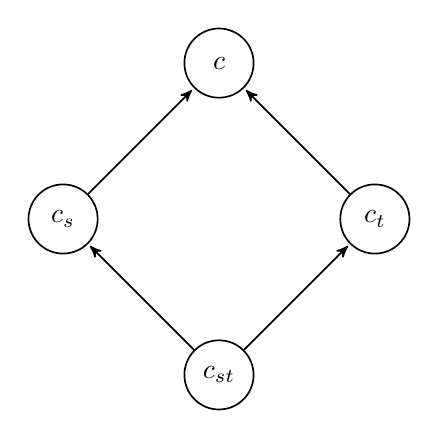
\begin{tikzpicture}[->,>=stealth',shorten >=1pt,auto,node distance=2.8cm, semithick]

    \node[state] (B)        {$c$};
    \node[state] (C) [below left of=B]  {$c_s$};
    \node[state] (D) [below right of=B] {$c_t$};
    \node[state] (E) [below left of=D]  {$c_{st}$};

    \path
    (C) edge node {} (B)
    (D) edge node {} (B)
    (E) edge node {} (C)
    (E) edge node {} (D);
\end{tikzpicture}  

\end{document}

%%% Local Variables:
%%% mode: latex
%%% TeX-master: t
%%% End:
